\documentclass[11pt,a4paper,twoside]{article}
\usepackage[utf8]{inputenc}
\usepackage[T1]{fontenc}

\usepackage{mathptmx}
\usepackage{datetime}
\usepackage[spanish, es-nolists]{babel}
\usepackage{amsmath}
\usepackage{amsthm}
\usepackage{amsfonts}
\usepackage{amssymb}
\usepackage{titlesec}
\usepackage{graphicx}
\usepackage{mathtools}

\decimalpoint

\usepackage{array}
\usepackage{float}
\usepackage[a4paper]{geometry}
\geometry{top=2.5cm, bottom=2cm, left=2.54cm, right=2.54cm}
\usepackage{fancyhdr}
\pagestyle{fancy}
\fancyhf{}  % Limpiar los encabezados y pies de página predeterminados
% Encabezados para páginas impares
\fancyhead[LE,RO]{\thepage} % En la izquierda de la página impar
\fancyhead[RE]{\textsc{Garbayo, I.}} % En la derecha de la página impar
% Encabezados para páginas pares
\fancyhead[LO]{\textit{Generación y optimización de código}}  % En la izquierda de la página par
\fancyfoot{}

\usepackage{color}
\usepackage{cancel}
\usepackage{ulem}
\usepackage{tcolorbox}
\usepackage{multirow}
\usepackage{tikz}
\usetikzlibrary{babel, arrows.meta, arrows, datavisualization, patterns}
\usepackage{multicol}
\usepackage{stackrel}
\usepackage{pdfpages}
\renewcommand{\labelitemi}{\textbullet}

\theoremstyle{definition}
\newtheorem{ejemplo}{\textbf{Exemplo}}
\newtheorem{ejer}{\textcolor{red}{\textbf{Exercicio}}}
\newtheorem{defi}{\textbf{Definición}}
\newtheorem{theorem}{\textbf{Teorema}}
\newtheorem{lema}{\textbf{Lema}}
\newtheorem{corol}{\textbf{Corolario}}
\newtheorem{prop}{\textbf{Proposición}}
\newtheorem{nota}{\textbf{\textit{Nota}}}

\renewcommand\qedsymbol{$\blacksquare$}

\usepackage{hyperref}
\hypersetup{
	colorlinks,
	citecolor=black,
	filecolor=black,
	linkcolor=black,
	urlcolor=black
}

\usepackage{enumitem}


\newcommand{\imagen}[1]{
	\begin{figure} [H] \centering
		\includegraphics[width=\textwidth]{#1}
	\end{figure}
}

\title{%
	\LARGE \textbf{Compiladores e Intérpretes} \\ \vspace*{1cm} \textbf{Práctica 1: Generación y optimización de código}
	\\ \Large \textbf{Optimizaciones del compilador en un producto de matrices}}
\author{\textsc{Ignacio Garbayo Fernández}}
\date{Universidade de Santiago de Compostela}

\setlength{\parskip}{5pt}

\usepackage{setspace}

%\onehalfspacing % Configura el interlineado a 1.5

\setlength{\parindent}{0.7cm}

\usepackage[hang, small,labelfont=bf,up,textfont=up]{caption}
\usepackage{hanging}
\usepackage{sectsty}

\sectionfont{\fontsize{14}{15}\selectfont}
\subsectionfont{\fontsize{12}{15}\selectfont}
\subsubsectionfont{\fontsize{12}{15}\selectfont}

\usepackage{titlesec}
\titleformat{\subsection}[block]{\normalfont\large\itshape}{\thesubsection}{1em}{}
\titlespacing*{\section}
{0pt}{\baselineskip}{0pt}
\titlespacing*{\subsection}
{0pt}{\baselineskip}{0pt}
\titlespacing*{\subsubsection}
{0pt}{\baselineskip}{0pt}

\usepackage[cache=false]{minted}
\definecolor{bg}{rgb}{.95, .95, .95}

\usepackage[backend=biber, style=ieee, sorting=nty]{biblatex}
\bibliography{references}


\begin{document}
	
	% PORTADA
	\maketitle
	\thispagestyle{empty}
	
	\vspace*{1cm}
	
	% ÍNDICE
	\renewcommand{\contentsname}{Índice} % Cambia el título
	\tableofcontents


	\newpage


	\section{Introducción}
	
	El objetivo de este experimento es analizar el impacto de las distintas optimizaciones del compilador GCC sobre un código ineficiente de multiplicación de matrices cuadradas en lenguaje \texttt{C}. El código realiza el producto de dos matrices de tamaño $n \times n$ utilizando tres bucles anidados sin ningún tipo de optimización algorítmica.
	
	El programa se compila con los niveles de optimización \texttt{-O0}, \texttt{-O1}, \texttt{-O2}, \texttt{-O3} y \texttt{-Os}, y se mide el tiempo de ejecución con precisión de nanosegundos. Además, se estudian las diferencias en el código ensamblador generado, el tamaño de los archivos de código objeto, los tiempos de ejecución y las aceleraciones obtenidas entre las versiones más eficientes.
	
	Este análisis permite observar cómo las optimizaciones del compilador afectan al rendimiento y a la eficiencia del código sin modificar el algoritmo subyacente.
	

	\section{Descripción de la técnica}
	
	Para la práctica, se propone estudiar el rendimiento de la siguiente porción de código.
	
	\begin{minted}[linenos, fontsize=\small, bgcolor=bg]{c}
for(j=0;j<Nmax;j++) { /* Producto matricial */
	for(i=0;i<Nmax;i++) {
		t=0;
		for (k=0;k<Nmax;k++) {
			producto(A[i][k],B[k][j],&r);
			t+=r; 
		}
		C[i][j]=t; 
	} 
}
	\end{minted}
	
	
	\subsection{Configuración del experimento}
	
	El objetivo del experimento es analizar el comportamiento de las diferentes optimizaciones del compilador, a saber: \texttt{O0}, \texttt{O1}, \texttt{O2}, \texttt{O3} y \texttt{Os}. Para esto, se prueba con un pequeño \textit{array} de valores de \texttt{N}. El \textit{array} se muestra en (\ref{eq:n}).
	
	\begin{equation}\label{eq:n}
		\begin{aligned}
			\texttt{N} = \left(
			\begin{matrix}
				100, & 300, & 500, & 600, & 700.
			\end{matrix}
			\right).
		\end{aligned}
	\end{equation}

	No se ha escalado en mayor medida el tamaño del problema, pues la definición estática en la pila de las matrices necesarias para la programación provocaba que se precisase más memoria de la disponible en la máquina. Además, definir las matrices como dinámicas empeoraba en gran medida la eficiencia de los accesos.

	Al ya efectuarse el experimento mediante un doble bucle sobre cada uno de los valores de \texttt{N} mostrados en (\ref{eq:n}), no es necesario definir un número \texttt{ITER} para evitar el ruido, como sí se hace en la Práctica 2 de la asignatura.

	Para cada valor de \texttt{N}, es fundamental ejecutar el algoritmo un número suficiente de veces, denotado por \texttt{REPS}, con el fin de obtener medidas de rendimiento representativas y estables. La variabilidad inherente al sistema ---debido a factores como la planificación del sistema operativo, el estado de la caché, o procesos en segundo plano--- puede provocar fluctuaciones significativas en los tiempos de ejecución individuales. Al repetir las mediciones y calcular posteriormente estadísticas como la \textbf{media}, la \textbf{desviación típica}, el \textbf{máximo} y el \textbf{mínimo}, se obtiene una caracterización más completa del comportamiento del algoritmo. Estas métricas permiten representar en las gráficas no solo la tendencia central, sino también la dispersión y los extremos del rendimiento, ofreciendo una visión más realista y robusta para comparar implementaciones o analizar cuellos de botella. Para este particular, \texttt{REPS} se fija a 100, un número suficientemente grande, como se comentó en clase.
		
	
	\section{Niveles de optimización de GCC}

	El compilador GCC proporciona distintos niveles de optimización que pueden activarse mediante las opciones \texttt{-O0}, \texttt{-O1}, \texttt{-O2}, \texttt{-O3} y \texttt{-Os}, como se muestra en \cite{gcc}. Cada uno de estos niveles activa diferentes transformaciones y análisis sobre el código fuente con el objetivo de mejorar su rendimiento o reducir su tamaño, a costa de aumentar el tiempo de compilación o dificultar la depuración.
	
	El nivel \texttt{-O0} es el predeterminado y está diseñado para acelerar la compilación y facilitar la depuración. No se realiza ninguna optimización sobre el código: se generan instrucciones prácticamente una a una a partir del código fuente. Esto permite una correlación directa entre el código fuente y el ejecutable, pero da lugar a un binario ineficiente y con tiempos de ejecución mayores.
	
	El nivel \texttt{-O1} introduce un conjunto básico de optimizaciones que buscan reducir tanto el tamaño como el tiempo de ejecución del código sin aumentar demasiado el tiempo de compilación. Entre las optimizaciones activadas en este nivel se incluyen:
	
	\begin{itemize}
		\item Eliminación de código muerto, es decir, instrucciones que nunca se ejecutan o cuyos resultados no se utilizan.
		\item Propagación de constantes, que sustituye expresiones por sus valores constantes cuando sea posible.
		\item Eliminación de operaciones redundantes, como comparaciones duplicadas o asignaciones innecesarias.
		\item Fusión de ajustes de pila consecutivos para mejorar la eficiencia en llamadas a funciones.
		\item Omisión del puntero de marco en funciones simples, lo que reduce el uso de registros.
	\end{itemize}

	Este nivel es especialmente adecuado para programas grandes generados automáticamente, donde se desea un equilibrio entre rendimiento y consumo de memoria durante la compilación.
	
	El nivel \texttt{-O2} amplía las optimizaciones anteriores y activa casi todas las que no suponen un compromiso directo entre tamaño y velocidad. Se añaden optimizaciones más complejas, como:
	
	\begin{itemize}
		\item Inlining parcial de funciones pequeñas o llamadas únicas, lo que evita la sobrecarga de llamadas.
		\item Hoisting de cargas adyacentes, que agrupa lecturas similares para reducir accesos a memoria.
		\item Reordenamiento de bloques de código y funciones para mejorar la localidad de instrucciones.
		\item Vectorización de bucles, que transforma operaciones escalares en operaciones vectoriales cuando es posible.
		\item Eliminación de punteros nulos redundantes y optimizaciones para cadenas de texto y cálculos de longitud.
	\end{itemize}

	\texttt{-O2} es probablemente el nivel más equilibrado en la mayoría de los casos reales, ya que mejora sensiblemente el rendimiento sin aumentar demasiado el tamaño del ejecutable.
	
	El nivel \texttt{-O3} activa todas las optimizaciones de \texttt{-O2} y añade otras aún más agresivas orientadas a maximizar la velocidad de ejecución, aunque esto puede aumentar considerablemente el tamaño del código generado. Entre las optimizaciones adicionales destacan:
	
	\begin{itemize}
		\item Desenrollado y reordenamiento de bucles, lo que permite aprovechar mejor la jerarquía de memoria.
		\item Separación y duplicación de caminos condicionales para mejorar la predictibilidad de las ramas.
		\item Vectorización avanzada con un modelo de costes dinámico para adaptar las transformaciones al hardware.
		\item Clonado de funciones para especializar comportamientos en contextos diferentes.
	\end{itemize}

	\texttt{-O3} puede producir importantes mejoras de rendimiento en código intensivo en cálculos, aunque no siempre es beneficioso para todos los programas.
	
	Finalmente, el nivel \texttt{-Os} está diseñado para minimizar el tamaño del ejecutable. Incluye todas las optimizaciones de \texttt{-O2}, excepto aquellas que tienden a aumentar el tamaño del código, como el alineamiento agresivo de funciones o bucles. Además:
	
	\begin{itemize}
		\item Se fuerza la inserción de funciones en línea solo si esto reduce el tamaño total del código.
		\item Se reorganiza el código para maximizar la reutilización de instrucciones y estructuras de control.
		\item Se ajusta el uso de memoria intermedia para reducir la huella del programa.
	\end{itemize}

	\texttt{-Os} es ideal para sistemas embebidos o programas donde el tamaño del binario es crítico.
	
	Cada nivel representa una estrategia diferente en cuanto a las prioridades del programador: depuración (\texttt{-O0}), compilación rápida (\texttt{-O1}), rendimiento general (\texttt{-O2}), rendimiento máximo (\texttt{-O3}) o tamaño mínimo (\texttt{-Os}).
	
	\section{Programación y código en ensamblador}
	
	\subsection{Arquitectura de compilación y ejecución}
	
	La compilación con la opción \texttt{-S} de GCC produce códigos fuente del ensamblador de la máquina mediante los que podemos analizar la traducción de las 2 estrategias. Se han ejecutado los códigos en una máquina ASUS Zenbook UX425EA 1.0, equipada con el sistema operativo Ubuntu 22.04.3 LTS x86\_64. Cuenta con un procesador Intel i7-1165G7 de 4 núcleos físicos de undécima generación, que funciona a una frecuencia de reloj de 2.80 GHz. Las direcciones de memoria ocupan 39 bits físicos y 48 bits virtuales.
	
	Cada núcleo dispone de 2 hilos de procesamiento, resultando en un total de 8 hilos. Dispone de 16 GiB de memoria RAM totales y de 4 niveles de memoria caché: L1d (192 KiB, 4 instancias), L1i (128 KiB, 4 instancias), L2 (5 MiB, 4 instancias) y L3 (12 MiB, 1 instancia). El TDP (\textit{Thermal Design Power}) es configurable entre 12 y 28 W. Se omite la inclusión de otros componentes como la tarjeta gráfica o de sonido porque no afectarán a los resultados de las pruebas. La versión del compilador utilizada es GCC 11.4.0.

	Con el fin de ejecutar las dos versiones en las mismas condiciones, el envoltorio de declaraciones y variables de medición previos a las llamadas correspondientes ha sido el que se muestra a continuación.
	
	Conviene mencionar que las mediciones se han efectuado utilizando la función \texttt{clock\_gettime()}, pues aporta una precisión de nanosegundos, necesaria para poder comparar las versiones compiladas con \texttt{O2}, \texttt{O3} o \texttt{Os}.
	
	\begin{minted}[linenos, fontsize=\small, bgcolor=bg]{c}
float A[Nmax][Nmax], B[Nmax][Nmax], C[Nmax][Nmax], t, r;
int i,j,k;

// Abrir fichero de escritura
if (argc < 2) { ... }
nombre_archivo = argv[1];
FILE* file = fopen(nombre_archivo, "a");
if (file == NULL) { ... }

// Calentamiento de la caché
for(i=0;i<Nmax;i++) { /* Valores de las matrices */
	for(j=0;j<Nmax;j++) {
		A[i][j]=(i+j)/(j+1.1);
		B[i][j]=(i-j)/(j+2.1);
	}
}

// Medir el overhead
clock_gettime(CLOCK_MONOTONIC, &overhead);
clock_gettime(CLOCK_MONOTONIC, &inicio);
// algoritmo
clock_gettime(CLOCK_MONOTONIC, &final);

// Cálculo de tiempos
tiempo_overhead = (inicio.tv_sec - overhead.tv_sec) + (inicio.tv_nsec
- overhead.tv_nsec) / 1e9;
tiempo = (final.tv_sec - inicio.tv_sec) + (final.tv_nsec - inicio.tv_nsec) / 1e9;
tiempo = tiempo - tiempo_overhead;

// Imprimir en el archivo
fprintf(file, "%d\t%.9f\n", Nmax, tiempo);
// Cerrar el archivo
fclose(file);
return 0;
	\end{minted}

	\subsection{Bucles}
	
	Vamos a centrarnos en la traducción de los bucles de \texttt{algoritmo}. La versión con \texttt{O0} presenta la estructura siguiente.
	
	\begin{minted}[linenos, fontsize=\small, bgcolor=bg]{nasm}
movl	$0, -3000032(%rbp)
jmp	.L10

.L15:
movl	$0, -3000036(%rbp)
jmp	.L11
.L14:
pxor	%xmm0, %xmm0
movss	%xmm0, -3000040(%rbp)
movl	$0, -3000028(%rbp)
jmp	.L12
.L13:
movl	-3000032(%rbp), %eax
movslq	%eax, %rdx
movl	-3000028(%rbp), %eax
cltq
imulq	$500, %rax, %rax
addq	%rdx, %rax
movss	-2000016(%rbp,%rax,4), %xmm0
movl	-3000028(%rbp), %eax
movslq	%eax, %rdx
movl	-3000036(%rbp), %eax
cltq
imulq	$500, %rax, %rax
addq	%rdx, %rax
movl	-3000016(%rbp,%rax,4), %eax
leaq	-3000044(%rbp), %rdx
movq	%rdx, %rdi
movaps	%xmm0, %xmm1
movd	%eax, %xmm0
call	producto
movss	-3000044(%rbp), %xmm0
movss	-3000040(%rbp), %xmm1
addss	%xmm1, %xmm0
movss	%xmm0, -3000040(%rbp)
addl	$1, -3000028(%rbp)
.L12:
cmpl	$499, -3000028(%rbp)
jle	.L13
movl	-3000032(%rbp), %eax
movslq	%eax, %rdx
movl	-3000036(%rbp), %eax
cltq
imulq	$500, %rax, %rax
addq	%rdx, %rax
movss	-3000040(%rbp), %xmm0
movss	%xmm0, -1000016(%rbp,%rax,4)
addl	$1, -3000036(%rbp)
.L11:
cmpl	$499, -3000036(%rbp)
jle	.L14
addl	$1, -3000032(%rbp)
.L10:
cmpl	$499, -3000032(%rbp)
jle	.L15
leaq	final(%rip), %rax
movq	%rax, %rsi
movl	$1, %edi
call	clock_gettime@PLT
	\end{minted}

	Esta versión no realiza optimización, por lo que se ve una traducción directa y detallada de cada paso del código C. En el código ensamblador se el bucle sobre \texttt{j}, el bucle sobre \texttt{i}, la inicialización de variables, las sumas parciales y el almacenamiento final de las mismas.

	Por otra parte, con \texttt{O1} destaca lo que se expone a continuación.
	
	\begin{minted}[linenos, fontsize=\small, bgcolor=bg]{nasm}
.L10:
subl	$1, %ecx
je	.L11
.L8:
movl	$500, %edx
jmp	.L12
	\end{minted}

	Este código ya omite completamente la estructura original explícita de tres bucles. Esto es indicativo de desenrollado parcial del bucle, fusión o simplificación de bucles y uso de registros para manejar iteraciones en vez de variables en memoria, como \texttt{-3000032(\%rbp)}. Posiblemente se está preparando un bucle que decrece (\texttt{subl \$1, \%ecx}), en vez de crecer. Es un inicio de optimización, pero aún mantiene la computación de la matriz C.
	
	Para \texttt{O2}, \texttt{O3} y \texttt{Os}, el ensamblador no contiene nada de código asociado a los bucles pues, al no utilizarse la matriz \texttt{C} durante el programa, su cálculo se omite. Esto es resultado de optimización por análisis de uso (DCE, \textit{Dead Code Elimination}). Como \texttt{C[i][j]} nunca se lee ni se imprime, el compilador concluye que calcularla es inútil, y elimina todo el bloque de bucles.
											
	
	\section{Resultados obtenidos}
	
	Los experimentos se han realizado teniendo en cuenta los parámetros \texttt{N} y \texttt{REPS} explicados en la sección 2. Las fases del experimento también se han introducido en la sección 4. En primer lugar, se realiza el calentamiento de la caché. Las matrices se llenan de valores flotantes (no enteros) para que ya puedna estar disponibles en niveles altos de la caché. 
	
	A continuación, se obtiene el \textit{overhead}, medición que tiene como objetivo estimar el tiempo que tarda en ejecutarse la propia medición del tiempo. Esto se aproxima calculando el tiempo que se tarda en usar \texttt{clock\_gettime()} dos veces seguidas.
	
	\subsection{Tamaño de códigos objeto}
	
	En el Cuadro \ref{tam} aparecen los tamaños de código objeto generado.
	
	\begin{table} [H] \centering
		\begin{tabular} {| c | c |}
			\hline
			\textbf{Optimización} & \textbf{Tamaño (bytes)} \\
			\hline
			\texttt{O0} & 16416 \\
			\hline
			\texttt{O1} & 16376 \\
			\hline
			\texttt{O2} & 16376 \\
			\hline
			\texttt{O3} & 16376 \\
			\hline
			\texttt{Os} & 16376 \\
			\hline
		\end{tabular}
		\caption{Tamaños de código objeto según tipo de optimización.}
		\label{tam}
	\end{table}

	La opción \texttt{O0} produce el código objeto más grande. Esto es esperable, ya que no aplica optimizaciones, por lo que incluye todo el código generado tal como aparece en el fuente, sin eliminar redundancias ni código innecesario.
	
	Por otra parte, \texttt{O1}, \texttt{O2}, \texttt{O3} y \texttt{Os} producen exactamente el mismo tamaño de código objeto. Esto sugiere que a partir de \texttt{O1}, el compilador ya elimina el código muerto (por ejemplo, el cálculo de la matriz \texttt{C} si no se usa). En este caso particular, las optimizaciones adicionales de \texttt{O2}, \texttt{O3} u \texttt{Os} no afectan al tamaño del código generado, posiblemente porque el código que queda es muy compacto o porque las mejoras son solo de rendimiento y no estructurales.

	
	\subsection{Tiempos de ejecución}
	
	El análisis realizado en la sección 4.2 sobre la traducción en código ensamblador se ve claramente reflejada en los tiempos de ejecución, que aparecen en la Figura \ref{tiempos}.
	
	\begin{figure} [H] \centering
		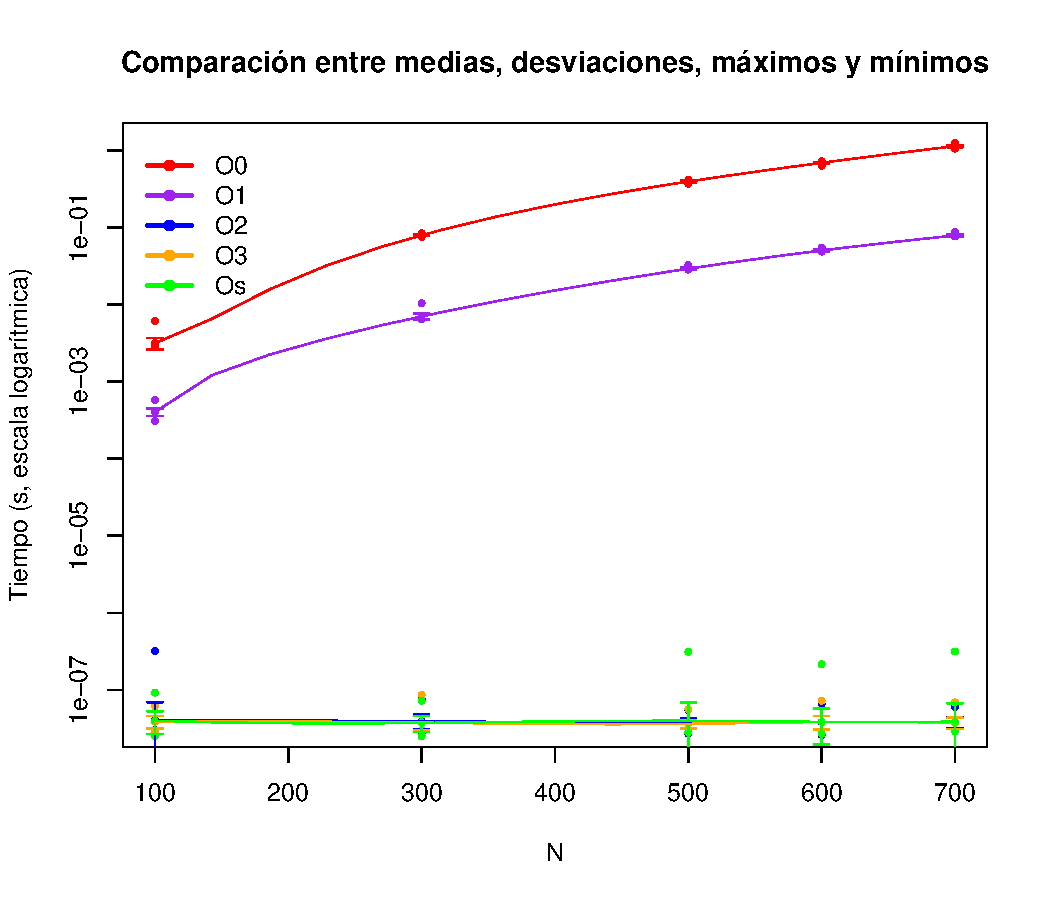
\includegraphics[width=.8\textwidth]{../graficas/tiempos.pdf}
		\caption{Tiempos de ejecución en función de la optimización.}
		\label{tiempos}
	\end{figure}

	En la Figura \ref{tiempos} se representa, para cada valor de \texttt{N} y cada optimización, un intervalo centrado en la media de los datos y con extremos la media $\pm$ la desviación típica de las observaciones. En puntos, habitualmente fuera de los intervalos, del mismo color, aparecen las observaciones mínima y máxima para cada combinación de las citadas. Esto es lo que se pidió en la presentación de la práctica.
	
	La gráfica ilustra claramente el impacto de las optimizaciones del compilador. Con \texttt{O0}, el código es fiel al original, completo pero lento. A partir de \texttt{O2}, el compilador elimina partes enteras del programa si no tienen efecto observable (como la asignación \texttt{C[i][j]}, que no se utiliza posteriormente). Esto implica que el tiempo de ejecución puede no reflejar el coste real del algoritmo si el compilador optimiza en exceso, como ocurre en este caso a partir de \texttt{O2}.
	
	Para este experimento, no tiene sentido analizar la aceleración. Las mejoras entre \texttt{O0}, \texttt{O1} y las demás se ve de forma clara en la Figura \ref{tiempos} y en las demás no se ejecuta código, por lo que los tiempos resultan en ocasiones incluso negativos (al hacer la resta con el \textit{overhead}).
	
	
	\section{Conclusiones}


\printbibliography
	
	

\end{document}